\section{Problem Statement}
Nowadays, the energy crisis is a constant theme because of the inflated energy prices \cite{energy_crisis}. Furthermore, huge energy consumption is a burden to the environment, as not all means of energy production are non-polluting. According to "Our World in Data"\cite{owidenergy}, in 2019, 63,3\% of eletrical energy production comes from fossil fuels. It is known that, in cities, street lamps are continuously switched on at night, most of the time unnecessarily glowing with its full intensity in the absence of any activities in the street.  This leads to a great waste of energy, also contributing to the increase in light pollution. As claimed by National Geographic \cite{light_pollution}, 83\% of world population lives under light-polluted skies. This is a problem since it alters the biochemical rhythms that normally flow with natural light levels and also endangers ecosystems by harming animals whose life cycles depend on dark.

With that in mind, the main objective of this project is the creation of a monitoring device, capable of controlling an intelligent street lamps network. These are capable of turning on only when they detect movement in the surroundings, adjusting their luminosity according to the needs of the surrounding environment. The device to be developed must be able to connect to all the sensors of each street lamp, must have knowledge of each operating conditions and location, and also must be able to control the street lamps individually, if necessary.

\section{Problem Statement Analysis}
In order to have a better and deeper understanding of the problem, it’s essential to identify the entities involved and their relationships. Using that analysis, a system diagram can be built, figure \ref{fig:Problem_statement_analysis}, relating the known entities and presenting some attributes.

\begin{figure}[ht]
	\centering
	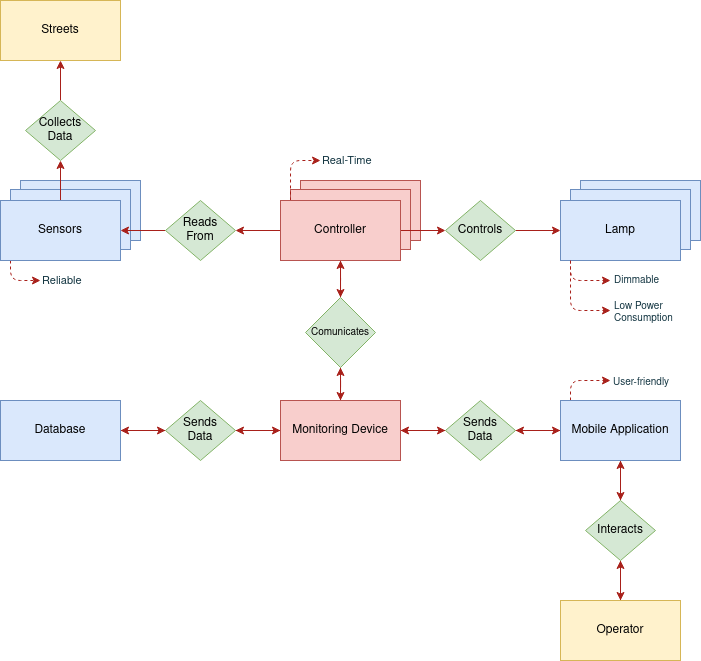
\includegraphics[width=1\textwidth]{Problem_statement_analysis}
	\caption{Problem Statement Analysis Diagram.}
	\label{fig:Problem_statement_analysis}
\end{figure}

The main purpose of this system is to control a network of smart street lamps, that is, turning them on when movement in the surroundings is detected and also adjusting their brightness according to the ambient light conditions. The system consists of a monitoring device, which communicates with various controllers. Each controller manages a single light pole, ensuring that its lamp lights up whenever motion is detected, through its sensors. The monitoring device receives and sends data to a database, which contains information about all lamp posts, and communicates with a mobile application. A responsible person for the lamp posts network, the operator, uses the application to obtain knowledge about this network. In addition, the monitoring device can also request each controller to turn on their lamp, regardless of whether or not there is movement in the vicinity of this pole.
